% chapter 2
\chapter{Datapath}
\label{chap:02_datapath}

\section{Structure}
As previously articulated, and as represented in detail with a representative schematic in Figure~\ref{fig:datapath}, the datapath segregates into five distinct phases. The initial phase, known as the \textbf{fetch stage}, is responsible for retrieving instructions from the Instruction RAM (IRAM). Subsequently, the \textbf{decode stage} is tasked with obtaining register values correlated with the addresses specified in the fetch stage and extending immediate values to 32 bits. Following this, the \textbf{execute stage} takes charge of performing all the arithmetic, logical, and shift operations. Subsequently the \textbf{memory stage}, acting as the fourth phase, manages read or write actions to the Data RAM (DRAM). Lastly, the \textbf{write back stage} is in charge of correctly routing the results generated either by the Arithmetic Logic Unit (ALU) or the DRAM itself. \\

\begin{figure}[!htbp]
    \centering
    %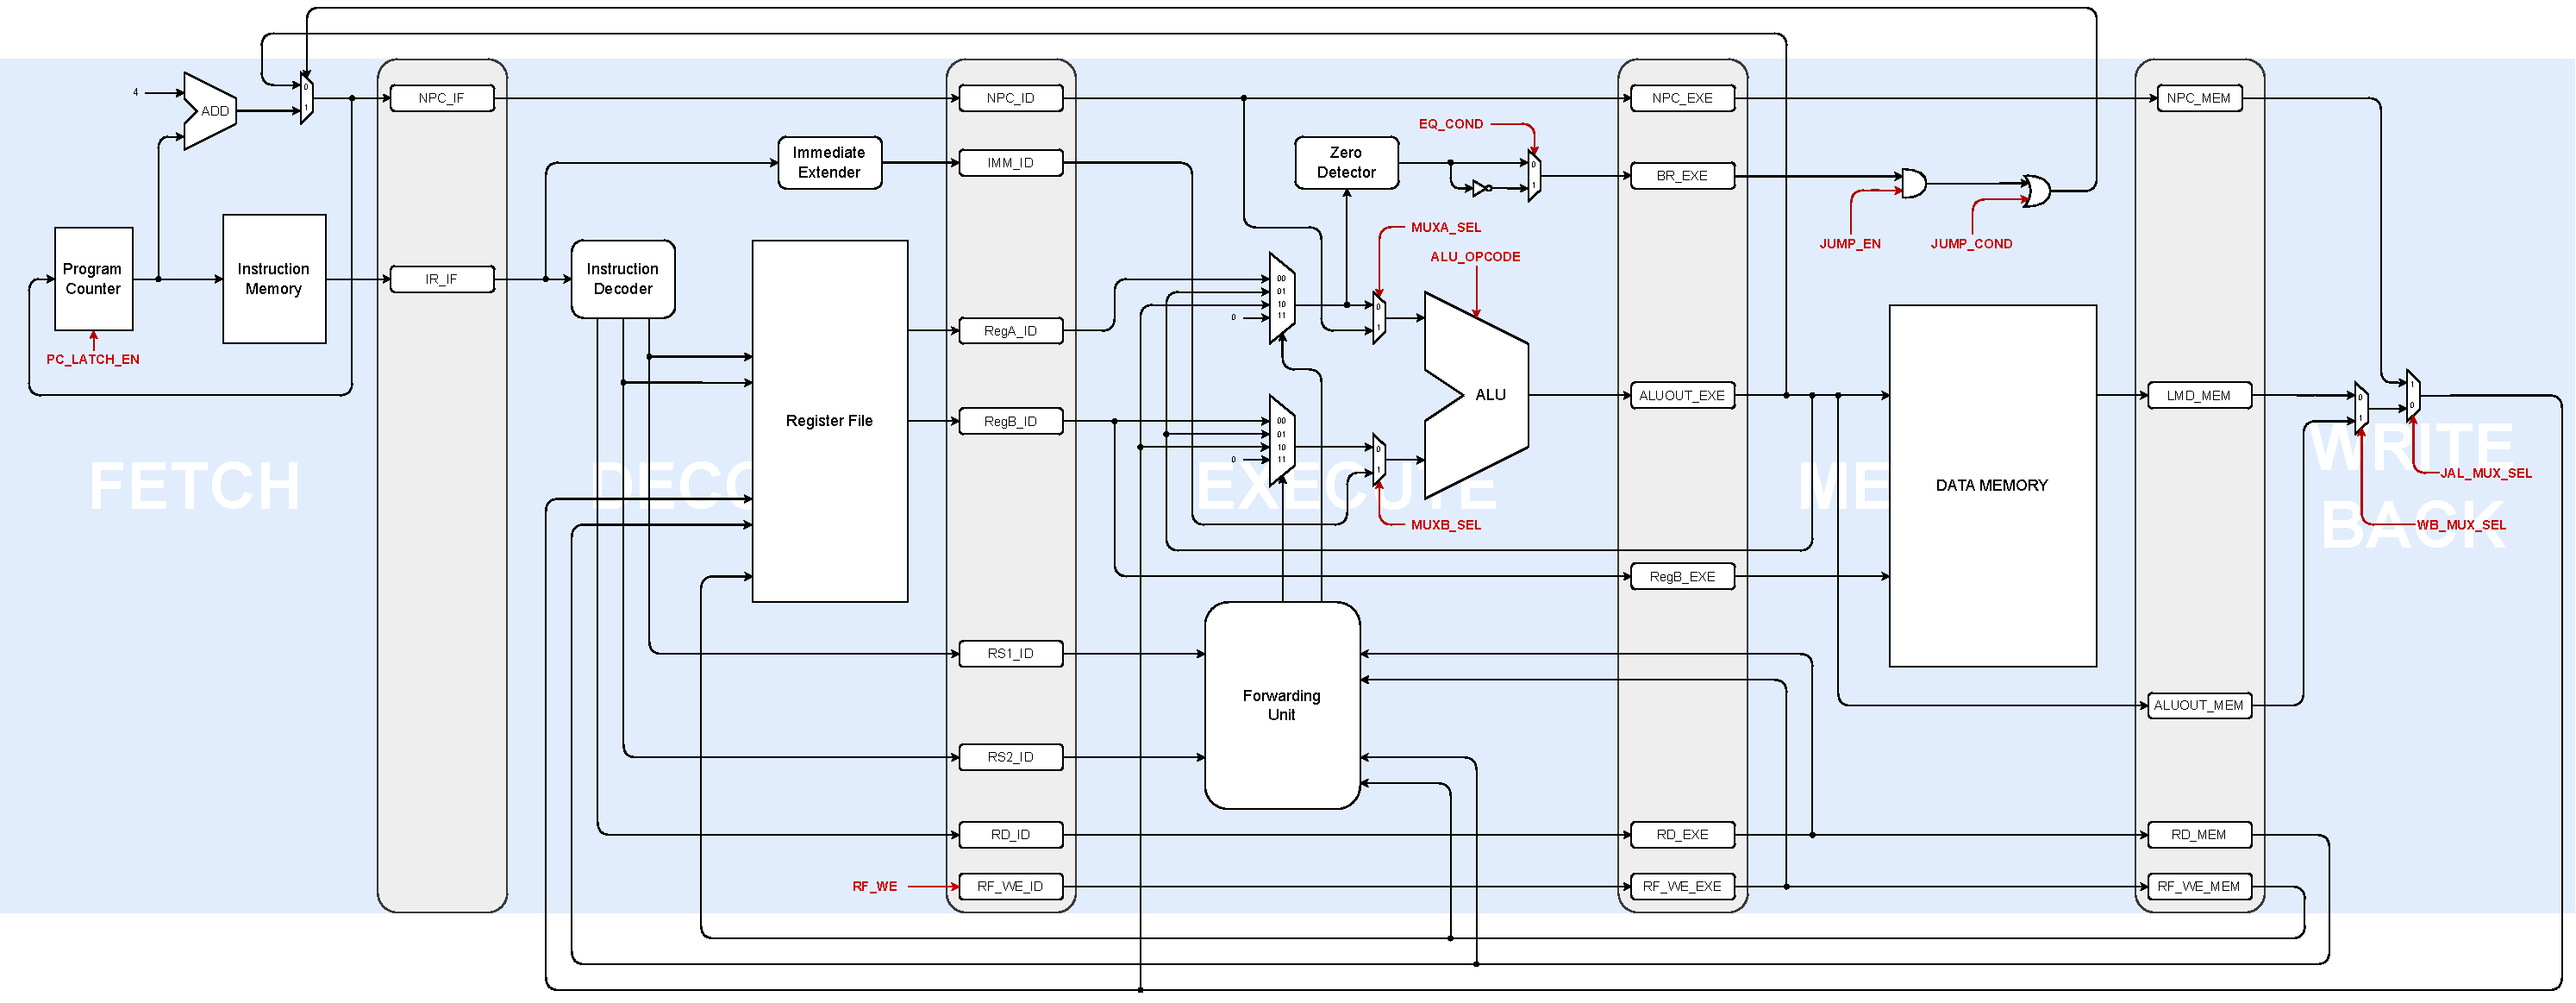
\includegraphics[width=0.95\textwidth]{source/figures/datapath.png}
    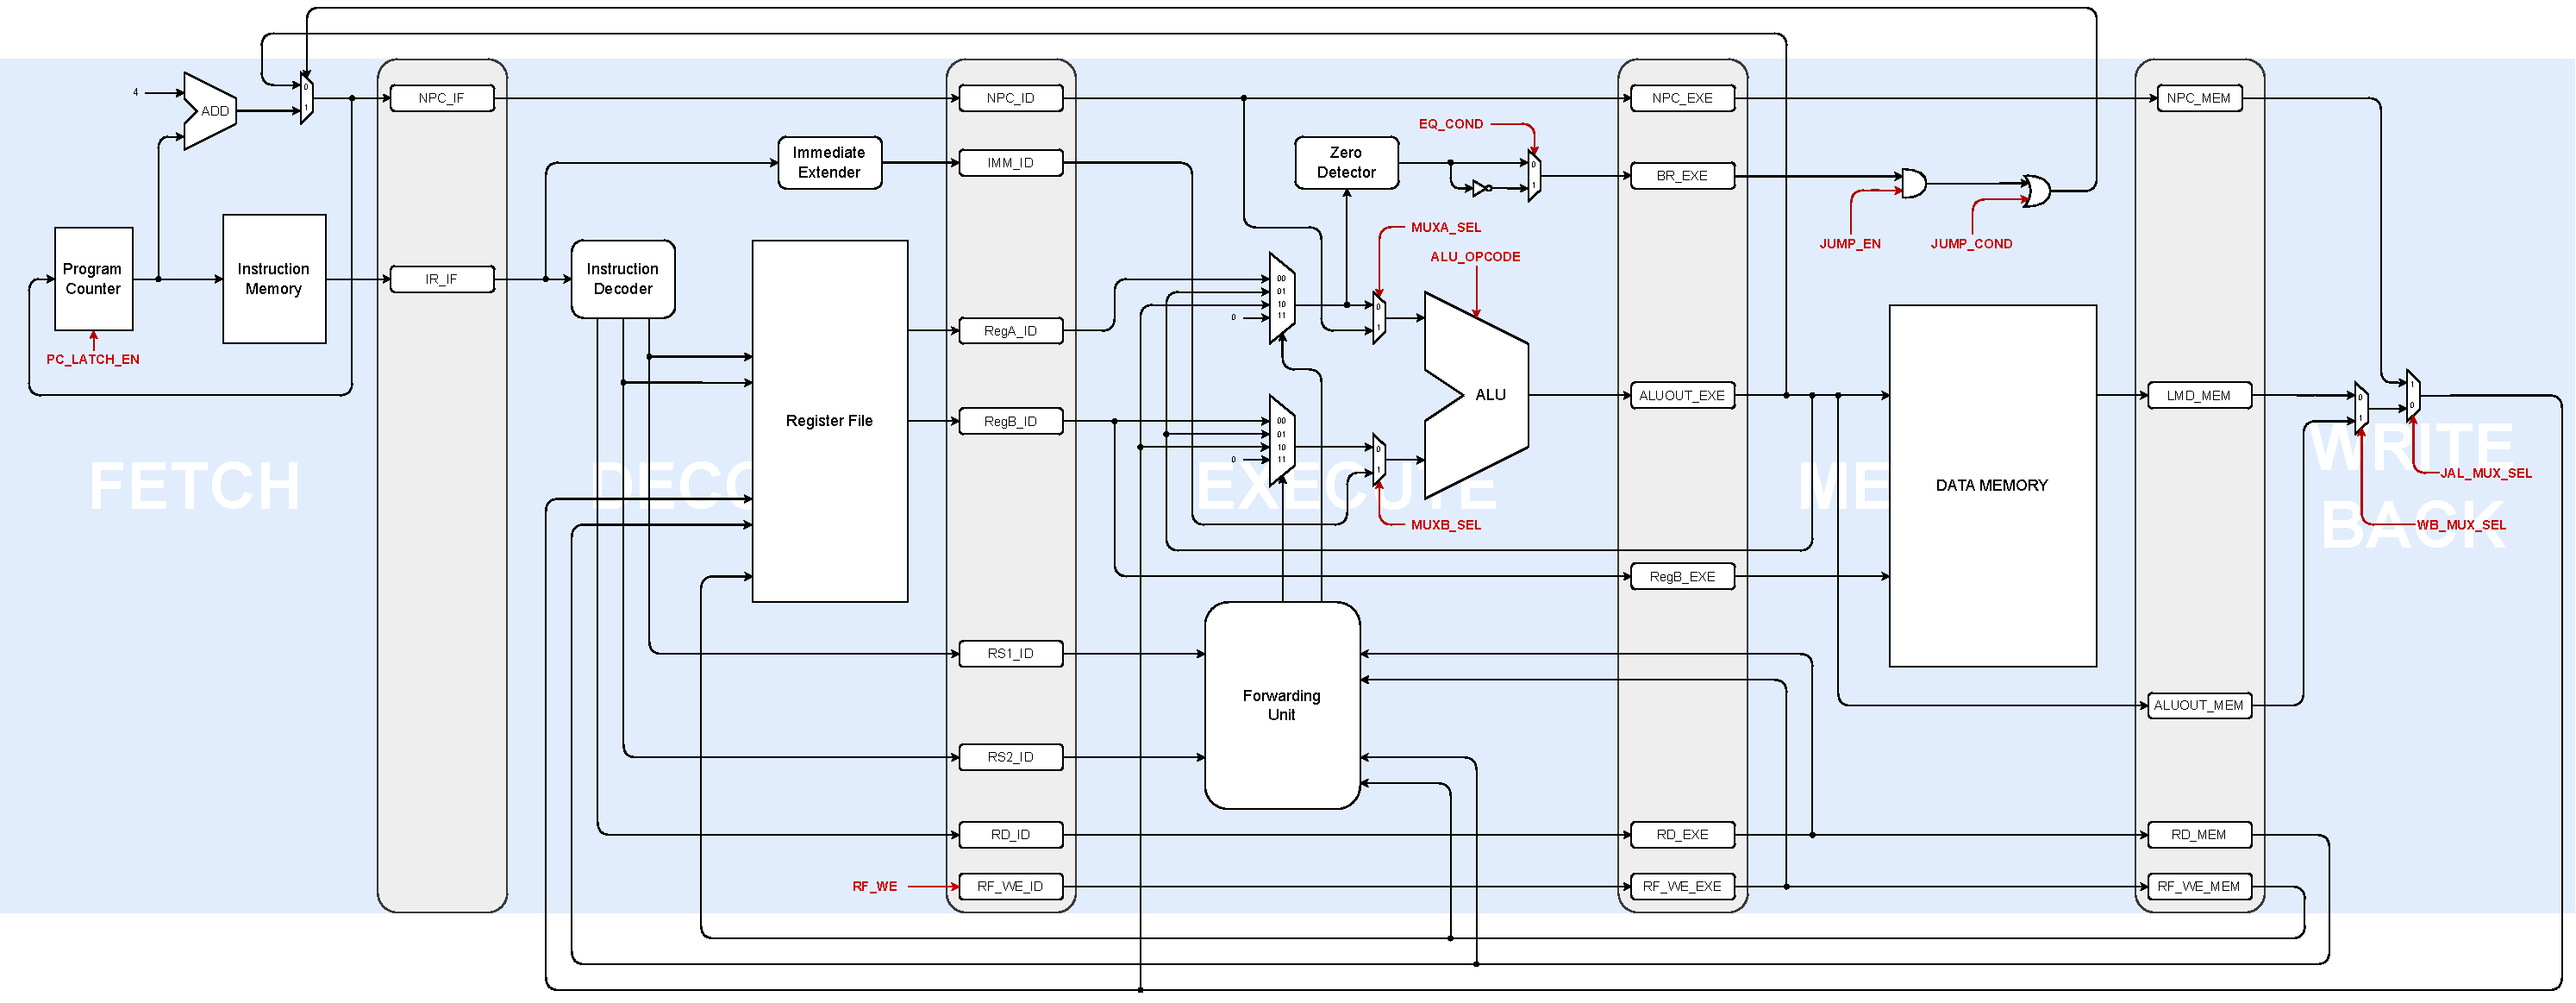
\includegraphics[angle=90,origin=c,width=0.6\textwidth]{source/figures/datapath.pdf}
    \caption{Datapath architecture}
    \label{fig:datapath}
\end{figure}

%----------------------------------------------------------------------------------------------------

\newpage
\section{Fetch Stage}
During the fetch stage, the next instruction to be executed is retrieved from the \textbf{Instruction Memory (IRAM)}, using the current address stored in the \textbf{Program Counter (PC)}. The instruction is then stored in the \textbf{Instruction Register (IR)} before proceeding to the next pipeline stage. In scenarios of sequential instruction execution, the PC is typically incremented by 4 to align with the 4-byte encoding standard of each instruction. In contrast, for control flow instructions like branches or jumps, the PC may be modified differently. Specifically, the \textbf{multiplexer} is activated in these cases, directing the output of the \textbf{Arithmetic Logic Unit} from the Memory stage to both the \textbf{Program Counter} and the \textbf{Next Program Counter Register}, as depicted in Figure~\ref{fig:01_fetch}.

\begin{figure}[!htbp]
    \centering
    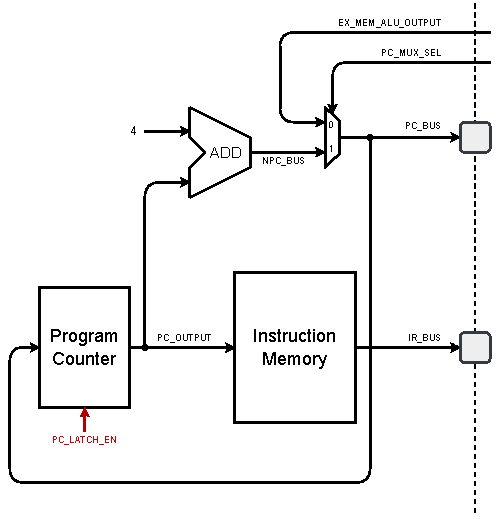
\includegraphics[width=0.55\textwidth]{source/figures/01_fetch.pdf}
    \caption{Fetch stage architecture}
    \label{fig:01_fetch}
\end{figure}

\subsection{Program Counter Register (PC)}
The Program Counter Register (PC) is a 32-bit register that holds the memory address of the instruction that is to be fetched and executed next. This register is updated continuously during the pipeline's operation to ensure smooth sequential instruction execution.

\subsection{Instruction Register (IR)}
The Instruction Register (IR) is another 32-bit register, which temporarily stores the instruction fetched from the Instruction Memory (IRAM). Once the instruction is loaded into the IR, it is forwarded to the decoding stage, where its opcode and operands are analyzed. Given the transient storage requirement for each fetched instruction, a latch-based D Register is used for implementing this component.

\subsection{Next Program Counter Register (NPC)}
The Next Program Counter Register (NPC) is a specialized 32-bit register designed to facilitate the forwarding of the Program Counter (PC) throughout the pipeline stages. This register is especially crucial when handling jump and branch instructions, as it can hold an alternative address to which control must be transferred. Like the Instruction Register, the NPC is implemented using a latch-based D Register.

\subsection{Adder}
This simple Adder calculates the address for the succeeding instruction by simply adding 4 to the current PC value \(PC + 4\). This is done to match the 4-byte instruction encoding standard, allowing for a seamless transition to the next instruction in the memory.

\subsection{Multiplexer}
This Multiplexer is used to choice between the next sequential address \(PC + 4\) and an alternative address provided by the Arithmetic Logic Unit (ALU). This component comes into play particularly during conditional branching or jumps, enabling the system to either continue with the sequential flow or divert to a different flow based on conditions met in the memory stage.

\paragraph{Additional Notes}
It's worth noting that while the Instruction Memory (IRAM) plays a critical role in the fetch stage by providing the instructions to be executed, it is not considered part of the datapath itself. IRAM is responsible for storing the entire instruction set that the DLX processor will execute, and its integration is essential for the pipeline's functioning. However a detailed discussion on the Instruction Memory will be covered in Chapter~\ref{chap:04_memories}, which is dedicated to memory systems.

%----------------------------------------------------------------------------------------------------

\newpage
\section{Decode Stage}
During the decode stage, as shown in Figure~\ref{fig:02_decode}, the pipeline prepares for the subsequent execution of the instruction initially fetched into the \textbf{Instruction Register (IR)}. The primary objective of this stage is to interpret the instruction and extract the operands and immediate values so that they can be utilized in the following stages of the pipeline. \\

At the heart of this operation is the \textbf{Instruction Decoder}, which breaks down the instruction to extract the register addresses that will act as operands for the upcoming operation. Working in concert with the decoder, the \textbf{Immediate Extender} performs sign-extension for immediate values. Complementing these components, the \textbf{Register File} stores the processor's registers, making these values accessible for the stages that follow.

\begin{figure}[!htbp]
    \centering
    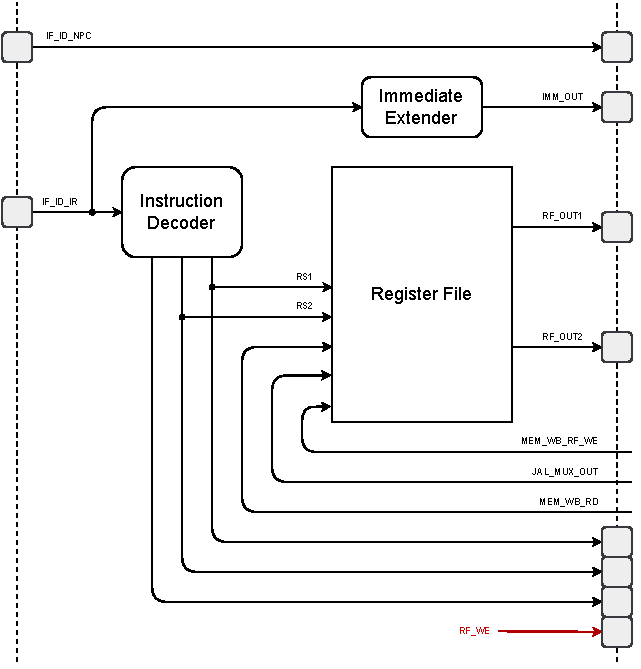
\includegraphics[width=0.7\textwidth]{source/figures/02_decode.pdf}
    \caption{Decode stage architecture}
    \label{fig:02_decode}
\end{figure}

\subsection{Instruction Decoder}
The Instruction Decoder takes the 32-bit instruction fetched into the Instruction Register (IR) and extracts the register addresses that will be used as operands for the upcoming operation, based on the last 6 bits that represent the opcode of the instruction. \\

It identifies the type of instruction, whether it's R-Type, I-Type, or J-Type, and retrieves the output addresses of the source registers (\texttt{RS1} and \texttt{RS2}) and the destination register (\texttt{RD}) that will be engaged in the actual operation. For instance, in the case of an R-Type instruction, all three fields are relevant. Conversely, for a standard \texttt{J} instruction, these fields may not be applicable, and they are set to zero, as previously shown in Figure~\ref{fig:instruction_format}. \\

The module also accommodates specificities in certain J-Type instructions: for example, when encountering a Jump and Link instruction (either \texttt{JAL} or \texttt{JALR}), the \texttt{RD} is automatically set to 31.

\subsection{Immediate Extender}
The Immediate Extender kicks in to perform sign-extension for immediate values. This ensures that immediate values, initially in either 16-bit or 26-bit formats, are accurately converted to a 32-bit format, enabling them to be treated as either signed or unsigned as the instruction dictates. \\

The Immediate Extender module is responsible for performing sign-extension of immediate values. This functionality ensures that immediate values, which may initially be in 16-bit or 26-bit formats, are accurately converted to a 32-bit format. The conversion allows these values to be treated as either signed or unsigned integers, in accordance with the specific instruction being executed. \\

This module determines the type of instruction, such as R-Type, I-Type, or J-Type, based on the opcode. For R-Type instructions, the immediate field is not applicable, and the module sets it to zero. On the other hand, J-Type instructions may contain a 26-bit immediate value, which undergoes sign-extension to align with the 32-bit architecture. I-Type instructions may involve either zero-extension or sign-extension of a 16-bit immediate value, depending on the particular operation being carried out. \\

For certain special cases like Load High Immediate (\texttt{LHI}), the higher 16 bits of the immediate value are used, while the lower 16 bits are zero-extended.

\subsection{Register File}
The Register File contains 32 general-purpose registers designed to hold runtime values for computation. These registers are 32-bit integers and can be addressed using 5-bit addresses, effectively ranging from \texttt{R0} to \texttt{R31}. \\

Certain registers receive special attention, as they are designated for specific roles in the processor's operation. For example, the \texttt{R0} register is read-only and is hardwired to always contain the value zero. On the other hand, the \texttt{R31} register is commonly used as the storage location for return addresses, particularly when executing Jump and Link instructions (\texttt{JAL} or \texttt{JALR}). Despite its specialized function, \texttt{R31} can also be employed for other general-purpose operations. \\

Reading from the Register File is always permitted, thereby obviating the need for a separate read-enable signal and simplifying the control logic. In contrast, a specific write-enable signal is generated by the Control Unit. This signal is carefully timed to ensure that data is written back into the register file only during the write-back stage. This synchronization is crucial for features controlled by the Forwarding Unit, which will be elaborated upon in a subsequent section. \\

The Register File is equipped with dual read data ports (\textbf{RD1} and \textbf{RD2}), enabling simultaneous reading from two different registers. This feature is essential for instructions that require two operands, as both can be fetched in a single clock cycle. Additionally, there is a single write data port that accepts the data to be written back into the register file. This data typically originates from the output of the final multiplexer in the write-back stage. \\

An active-low reset signal is also integrated into the design. When triggered, this signal clears the contents of all the registers. This functionality is particularly useful for initialization purposes or in situations requiring a rapid state reset.

%----------------------------------------------------------------------------------------------------

\newpage
\section{Execution Stage}
As illustrated in Figure~\ref{fig:03_execute}, the execution stage is responsible for accurately routing requisite operands to the \textbf{Arithmetic Logic Unit (ALU)} for a variety of computational tasks, ranging from basic arithmetic to bitwise logical operations. To ensure the correct operands are supplied to the ALU, a tree structure of multiplexers in conjunction with the \textbf{Forwarding Unit} manages the delivery of operands from the two subsequent pipeline stages. This is particularly important for cases where the results have not yet been written back into the Register File. Additionally, a specialized module called \textbf{Zero Detector} is tasked with verifying whether the first operand is zero, thus preparing the pipeline for potential conditional branches.

\begin{figure}[!htbp]
    \centering
    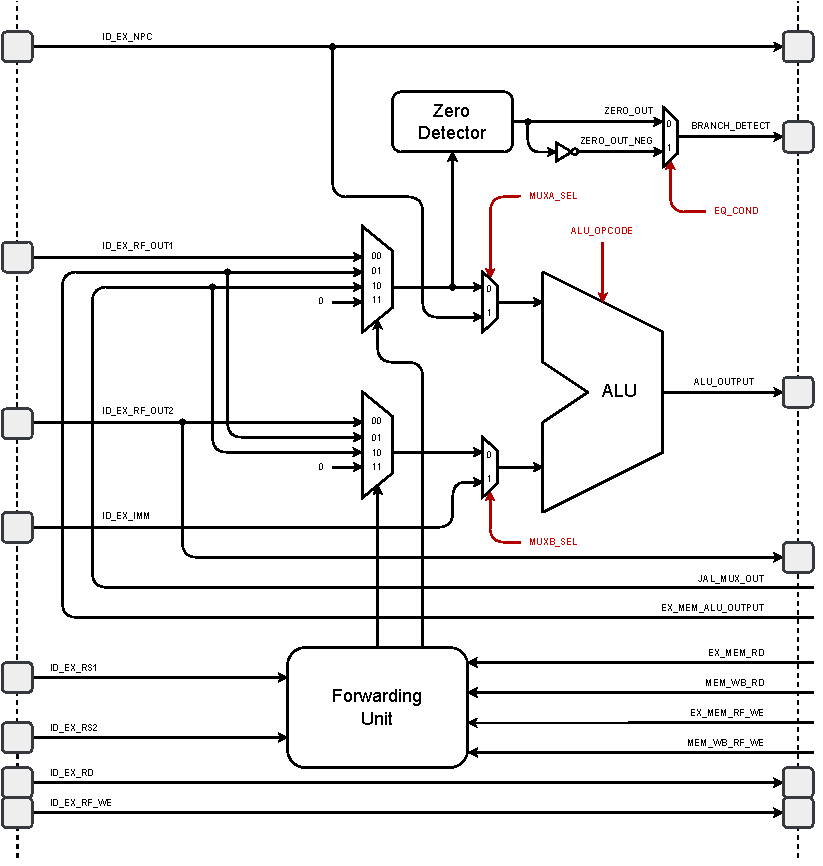
\includegraphics[width=0.9\textwidth]{source/figures/03_execute.pdf}
    \caption{Execute stage architecture}
    \label{fig:03_execute}
\end{figure}

\subsection{Arithmetic Logic Unit (ALU)}
The ALU, shown in Figure~\ref{fig:alu}, serves not only as the computational core of the execution stage but also as the pivotal computational component of the entire architecture. It is designed to handle a variety of operations, including both signed and unsigned arithmetic. The ALU receives two 32-bit operands along with a signal that specifies the operation type, and produces a single 32-bit output accordingly. \\

The ALU's versatility is attributed to several internal functional components that have been incorporated into the project. These include:

\begin{itemize}%[nosep]
    \item an adder module based on the \textbf{Pentium 4 Adder}, responsible for adding or subtracting operands;
    \item a specialized \textbf{Comparator Unit} for comparing both signed and unsigned numbers;
    \item a specialized \textbf{Logic Unit} for performing bitwise AND, OR and XOR operations between operands;
    \item two distinct \textbf{Barrel Shifters} for executing arithmetic and logic shifts;
    \item a \textbf{Radix-4 Booth Multiplier} for multiplication operations.
\end{itemize}

\begin{figure}[!htbp]
    \centering
    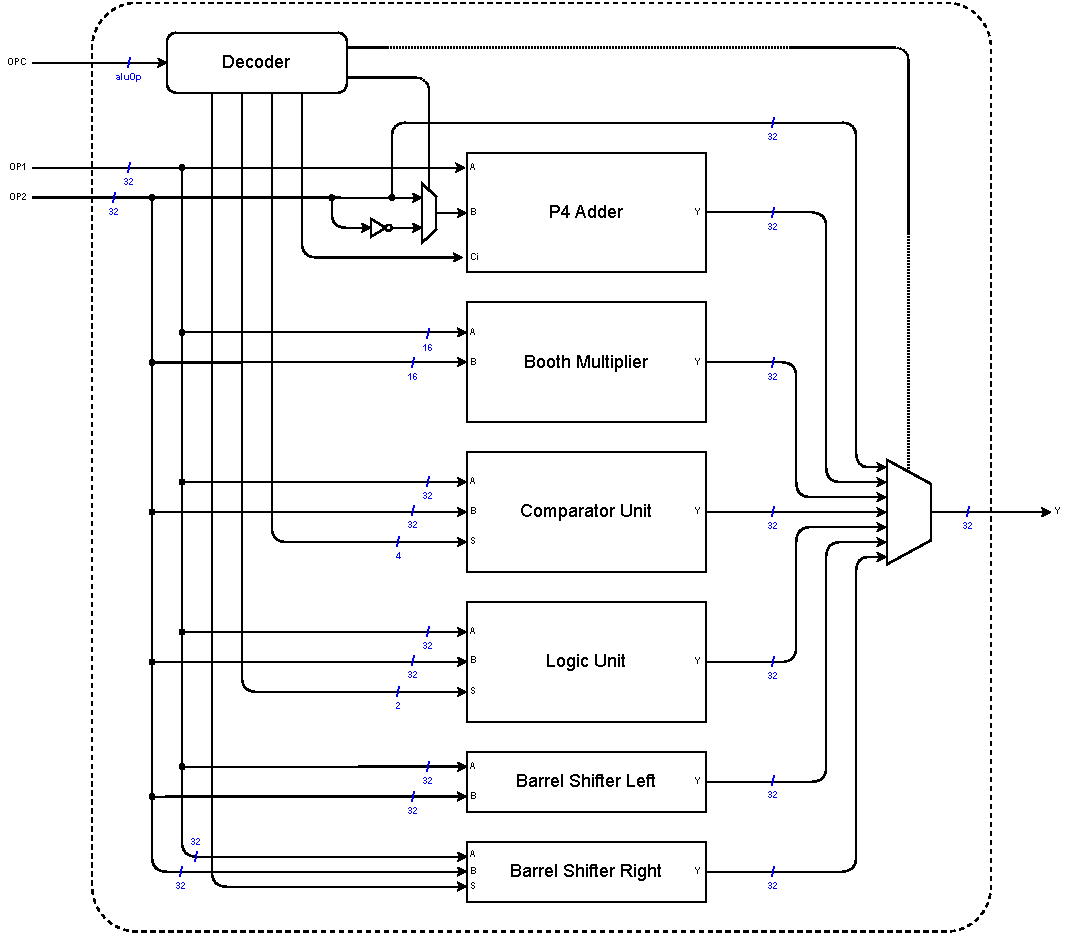
\includegraphics[width=1\textwidth]{source/figures/alu.pdf}
    \caption{Arithmetic Logic Unit (ALU) architecture}
    \label{fig:alu}
\end{figure}

Each of these components can handle both R-type operations, where values are sourced from the Register File, and I-type operations, where values are retrieved from the Register File as well as the Immediate field of the instruction being executed. Furthermore, the ALU also supports the computations required for generating the destination addresses for J-type instructions.

\subsubsection{Pentium 4 Adder}
The Pentium 4 Adder is a specialized 32-bit arithmetic unit capable of performing both addition and subtraction operations seamlessly. This adder builds upon the foundational netlists developed during laboratory sessions and is fundamentally divided into two primary subcomponents: the \textbf{Sum Generator} and the \textbf{Carry Generator}.

\begin{itemize}%[nosep]
    \item \textbf{Carry Generator}: computes the intermediate bits and the final carry bit.
    \item \textbf{Sum Generator}: produces the final sum of the operands by combining the input operands and the intermediate carries.
\end{itemize}

It is worth noting that the design of the P4 Adder emphasizes parallelism, utilizing both the Sum Generator and the Carry Generator in tandem. This approach not only increases speed by reducing the ripple effect commonly observed in simpler adders but also boosts operational efficiency.

\subsubsection{Comparator Unit}
The Comparator Unit provides support for executing a variety of comparison operations. These operations include \textit{less than} ($<$), \textit{greater than} ($>$), \textit{less than or equal to} ($\leq$), \textit{greater than or equal to} ($\geq$), \textit{equal to} ($=$), and \textit{not equal to} ($\neq$). Furthermore, the module is capable of handling both signed and unsigned operand comparisons. \\

The core functionality is governed by a 4-bit selector signal, which determines the type of comparison operation to be carried out. Depending on the value of this selector, the module performs the appropriate comparison between the two 32-bit operands and generates a 32-bit output to represent the result. Notably, the output is not a single-bit flag; instead, it is a full 32-bit word. This design choice maintains consistency with the data bus width and allows for the possibility of chaining with other operations.

\subsubsection{Logic Unit}
Designed for the execution of bitwise logical calculations, specifically \texttt{AND}, \texttt{OR}, and \texttt{XOR}, the Logic Unit employs a 2-bit selector signal to choose the operation to be carried out. \\

If the selector signal reads "00" the unit conducts a bitwise \texttt{AND} operation on the operands. If the selector signal shows "01" the unit performs a bitwise \texttt{OR} operation and for "10" it carries out a bitwise \texttt{XOR} operation. Should the unit receive an invalid selector signal, it is configured to return a default 32-bit zero output.

\subsubsection{Barrel Shifters}
Within the ALU, two types of barrel shifters are incorporated to execute both left and right shifts. In the case of the latter, both logical and arithmetic shifts are supported.

\begin{itemize}
    \item \textbf{Barrel Shifter Left (BSL)}: this module performs the left-shift operation on the first operand by a number specified by the second operand. The leftmost bits are discarded, and `0's are filled into the rightmost positions.
    
    \item \textbf{Barrel Shifter Right (BSR)}: this module performs the right-shift operation on the first operand by a number specified by the second operand. When executing a logical shift, `0's are introduced on the left. In contrast, during an arithmetic shift, the MSB (sign bit) is retained to ensure that the sign of the number remains unchanged. A shift type identifier is used to determine whether the shift is logical or arithmetic.
\end{itemize}

Both modules are structurally defined, and their architectural design employs a sequence of multiplexers. This design approach eliminates the need for iterative shifting one bit at a time, offering a significant speed advantage, especially for larger shifts.

\subsubsection{Radix-4 Booth Multiplier}
This project introduces a 32-bit signed integer multiplier based on the Booth's Multiplication Algorithm. The multiplier takes in two 16-bit operands and during each step of the partial multiplication process, the first operand is shifted one position, while the second operand is grouped into 3-bit segments. The summation of these partial products is executed using a tree-structured arrangement of Ripple-Carry Adders (RCA).

\paragraph{Booth's Multiplication Algorithm}
Booth's multiplication technique aims to optimize the multiplication process by reducing the number of partial products required. A sequence of consecutive `1's in a binary number can be replaced by generating a carry-out coupled with a subtraction at the least significant bit of the string. Mathematically, this is expressed as:
\[
\sum_{n=0}^{N-1} 2^n = 2^N - 1
\]

For example, \(0111_2\) can be re-expressed as \(1000_2 - 0001_2\). Similar methods can be applied to sequences of `1's appearing at other positions in a number by appropriately left-shifting the result.  \\

This optimization enables the reduction of the number of partial products involved in the multiplication. In this approach, the multiplier is represented in radix-4, allowing for digits between 0 and 3, as opposed to just 0 and 1. This halves the number of partial products needed since each multiplication operation now processes two bits at a time. However, multiplying by 3 presents a challenge, unlike multiplying by 0, 1, or 2, which only require simple shifts. To sidestep the difficulty of multiplying by 3, Booth's observations are applied to recode the digit set to include 2, 1, 0, -1, and -2. Positive digits yield simple partial products, whereas negative digits are handled by subtraction instead of addition, as shown in Table~\ref{tab:booth_encoding}. \\

\begin{table}[!htbp]
    \centering
    \begin{tabular}{|c|c|c|c|}
        \hline
        \( Bi+1 \) & \( Bi \) & \( Bi-1 \) & \( E2i \) \\
        \hline
        0 & 0 & 0 & 0 \\
        0 & 0 & 1 & \( A \) \\
        0 & 1 & 0 & \( A \) \\
        0 & 1 & 1 & \( 2A \) \\
        1 & 0 & 0 & \( -2A \) \\
        1 & 0 & 1 & \( -A \) \\
        1 & 1 & 0 & \( -A \) \\
        1 & 1 & 1 & 0 \\
        \hline
    \end{tabular}
    \caption{Booth Encoding Algorithm Table}
    \label{tab:booth_encoding}
\end{table}

\subsection{Forwarding Unit}
The Forwarding Unit serves as an essential component in enhancing pipeline efficiency and mitigating data hazards, specifically \textbf{read-after-write (RAW)} dependencies. It operates by identifying data dependencies between forthcoming instructions and instructions still in the pipeline but whose results have been fully computed. \\

This unit employs a comparison between register source encodings into the execution stage with those present in the memory and write-back stages. A match signifies a pending operand, already computed but not yet stored, that is required by the instruction decoded in the previous clock cycle. \\

Upon recognizing such data dependencies, the Forwarding Unit eliminates the need for \textbf{pipeline stalls} by routing the already-computed data directly to the required ALU input. This is achieved via a secondary set of multiplexer interconnections, as represented in the Figure~\ref{fig:03_execute}. In doing so, the Forwarding Unit ensures that each computation utilizes the correct, most up-to-date data, allowing for an optimized execution pipeline.

\subsection{Zero Detector}
In this architecture, the Zero Detector module plays a critical role in conditional \textbf{branching instructions}. It examines the first operand to determine whether all its bits are set to zero. This functionality significantly aids in evaluating branch conditions such as \texttt{BEQZ} and \texttt{BNEZ}. By quickly establishing the \textbf{zero condition}, the Zero Detector expedites the decision-making process for branching.

\subsection{Multiplexers}
Five multiplexers are employed within the execution stage:
\begin{itemize}
    \item \textbf{Two 32-bit 4-to-1 multiplexers} are responsible for selecting the first input for subsequent multiplexers. These are controlled by the Forwarding Unit, which allows for the selection of content originating from either the Register File in the previous stage, the memory stage, or the write-back stage.
    \item \textbf{Two 32-bit 2-to-1 multiplexers} serve to select the actual input value for the ALU. The choices are between the outputs of the preceding 4-to-1 multiplexers or, depending on their respective connections to the ALU, either the Next Program Counter value or the 32-bit sign-extended immediate value from the previous stage. These multiplexers are both governed by signals generated by the Control Unit.
    \item \textbf{A single-bit 2-to-1 multiplexer} that, depending on the type of branch to be executed (\texttt{BEQZ} or \texttt{BNEZ}), outputs either the output of the Zero Detector or its negated version.
\end{itemize}

%----------------------------------------------------------------------------------------------------

\newpage
\section{Memory Stage}
The memory stage functions as the fourth stage of the pipeline and serves as a straightforward segment for managing data as shown in Figure~\ref{fig:04_memory}. In this stage, data is either read from or write into the \textbf{data memory}, accessible solely through load and store operations. Additional \textbf{logic ports} are employed here to handle branch and jump conditions, as well as to control the multiplexer in the fetch stage.

\begin{figure}[!htbp]
    \centering
    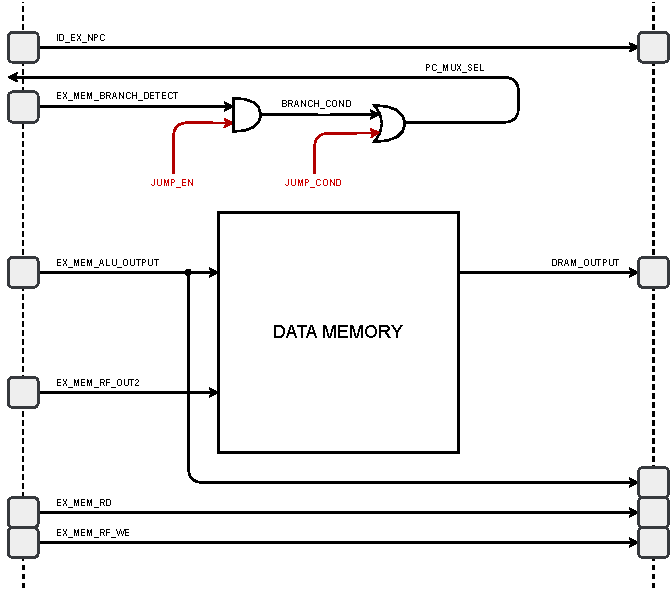
\includegraphics[width=0.8\textwidth]{source/figures/04_memory.pdf}
    \caption{Memory stage architecture}
    \label{fig:04_memory}
\end{figure}

\subsection{Logic Ports}
Two simple logic ports are utilized within the memory stage to manage jumps and branches effectively:
\begin{itemize}
    \item An \textbf{AND logic gate} is used in conjunction with a signal generated by the Control Unit. This signal becomes active exclusively during the execution of \texttt{BEQZ} or \texttt{BNEZ} instructions, allowing the branch condition to be forwarded to the subsequent logic stage if satisfied.
    \item An \textbf{OR logic gate} is responsible for generating the signal that directs the multiplexer in the fetch stage to select the next address for the Program Counter. This gate outputs a one either when the branch condition from the preceding stage is met or when the Control Unit's signal, designated for unconditional jumps, is activated.
\end{itemize}

\paragraph{Additional Notes}
Similar to the role of the Instruction Memory (IRAM) in the fetch stage, the Data Memory (DRAM) is crucial in the pipeline but is not inherently a part of the datapath. The DRAM functions within the memory stage, where it manages read or write operations as instructed by the pipeline. Essentially, DRAM serves as the storage hub for data that the DLX processor will manipulate throughout its operation. Unlike the IRAM, which stores only instructions, the DRAM accommodates data that can be both read from and written into. This flexibility makes it instrumental for the load and store operations performed in the memory stage. A comprehensive discussion on the Data Memory will also be covered in Chapter~\ref{chap:04_memories}, which focuses on memory systems in greater detail.

%----------------------------------------------------------------------------------------------------

\newpage
\section{Write-Back Stage}
The write-back stage serves as the phase in which the computational results are stored back into the designated register, as identified during the decode stage of the instruction pipeline. A two-level multiplexer tree is utilized here, as illustrated in Figure~\ref{fig:05_writeback}, to deliver the value required by the current instruction to the system. The write-enable signal, originally generated by the Control Unit, is routed to the Register File at this stage to facilitate the acceptance of the new value.

\begin{figure}[!htbp]
    \centering
    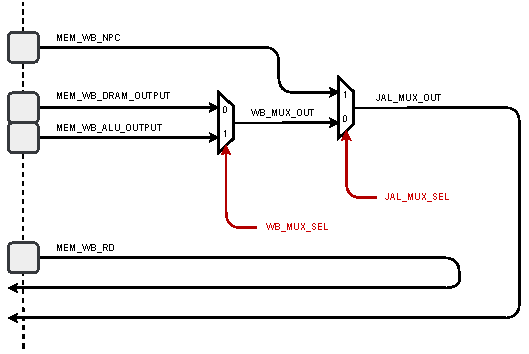
\includegraphics[width=0.6\textwidth]{source/figures/05_writeback.pdf}
    \caption{Write-Back stage architecture}
    \label{fig:05_writeback}
\end{figure}

\subsection{Multiplexers}
A straightforward hierarchy comprising two 32-bit 2-to-1 multiplexers is utilized in this stage:
\begin{itemize}
    \item The \textbf{first-level multiplexer}, controlled by a specific signal generated by the Control Unit, selects between the output of the ALU and the output from the DRAM in the event that a load operation (\texttt{LW}) has been executed.
    \item The \textbf{second-level multiplexer}, similarly governed by a dedicated signal from the Control Unit designed for handling jump-and-link instructions like \texttt{JAL} or \texttt{JALR}, chooses between the output of the preceding multiplexer and the value of the Next Program Counter that has been forwarded to this stage.
\end{itemize}
